
\section{Applications}


In this section, we chose four use cases to illustrate \biochem's capabilities in terms of functionality and usability, from basic operations to more advanced applications, while highlighting the advantages of using Julia for bioinformatics tasks.
We begin with a simple example to show the creation and usage of core structures. Next, we compare two different configurations of the same molecule. Finally, we want to demonstrate the elegance of Julia code in comparison to C++ in the context of \ball\ and \biochem\. In the last application, we briefly introduce the accompanying visualization tool \bioviz that has been developed alongside the \biochem\ framework.
 \begin{figure*}[t]
	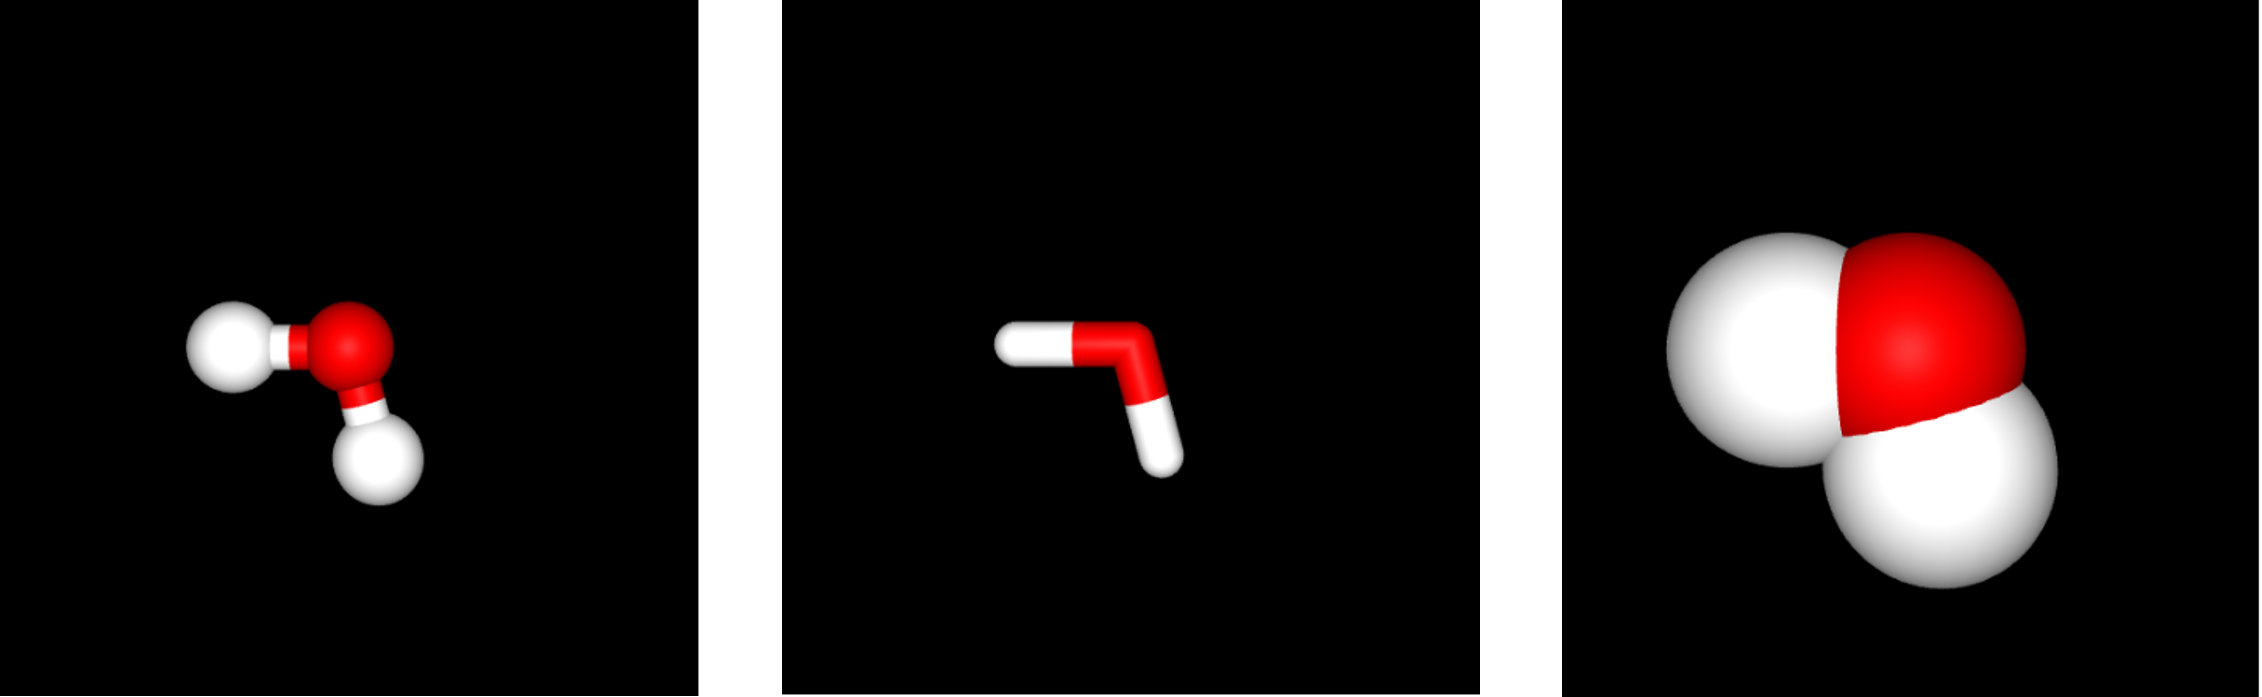
\includegraphics[width=18cm]{gfx/biovis-2.png}
	\caption{\bioviz supports three models:  \texttt{ball-and-stick} \textit{(left)}, \texttt{stick} \textit{(center)} and \texttt{van-der-waals} \textit{(right)} representation of the water molecule as generated by the code listing~\ref{lst:code-water}.}
	\label{fig:biochem_water}
\end{figure*}

\subsection{Generating a water molecule}


The core of \biochem\ is represented in a class diagram (Figure~\ref{fig:biochem_uml}), which illustrates the framework's intuitive design and straightforward component interactions as can be seen in code listing~\ref{lst:code-water}. 
\begin{lstlisting}[
	language = Julia, 
	numbers=left, 
	label={lst:code-water}, 
	caption={Intuitive usage of \biochem\ core components}
	]
using BiochemicalAlgorithms
using BiochemicalVisualization
	
sys = System() 
h2o = Molecule(sys)
	
o1 = Atom(h2o, 1, Elements.O, radius = 1.40f0)
h1 = Atom(h2o, 2, Elements.H, radius = 1.10f0)
h2 = Atom(h2o, 3, Elements.H, radius = 1.10f0)
	
h1.r = [1, 0, 0]
h2.r = [cos(deg2rad(105)), sin(deg2rad(105)), 0]

Bond(h2o, o1.idx, h1.idx, BondOrder.Single)
Bond(h2o, o1.idx, h2.idx, BondOrder.Single)
	
println("Number of atoms: ", natoms(h2o))
println("Number of bonds: ", nbonds(h2o))
	
ball_and_stick(sys)	
stick(sys)
van_der_waals(sys)
\end{lstlisting}

We have carefully chosen intuitive names for classes representing molecular entities and related functionalities. The \texttt{System} class serves as the central element of any application. If not explicitly created, a default system is generated automatically. Atoms can be created along with their corresponding bonds and will automatically be incorporated in the defined system. The resulting system, containing a water molecule in this example, can be visualized using the \bioviz\ tool (Figure~\ref{fig:biochem_water}). More details about the visualization capabilities are provided in the subsequent section of the paper. \\
This approach emphasizes ease of use and functionality, two of the key design goals mentioned earlier for \biochem. The intuitive interface and automatic system generation contribute to RAD, another stated goal of the framework.



\subsection{RMSD computation and Application of Amber}

This example demonstrates the use of \biochem for a common task in structural analysis: comparing two (or more) molecular structures. The process involves several steps (see code listing~\ref{lst:rmsd-and-amber}):
\begin{itemize}
	\item Loading structures: Two \pdb s are loaded into a \texttt{Vector} of \texttt{System}, rather than a single system as in the previous example.
	\item Preprocessing: The systems are preprocessed using the functionalities provided by the \texttt{FragmentDB} interface, a database containing known fragments of molecules: 
	\begin{itemize}
		\item Normalizes different naming standards
		\item Reconstructs missing parts of molecules
		\item Creates bonds (as the PDB format often lacks complete bond information)
	\end{itemize}
	\item Force field application: Each structure is applied to a molecular force field, specifically the Amber force field, and the energy of each system is computed.
	\item Structure mapping: The structures, which are different configurations of the same molecule, are mapped onto each other.
	\item RMSD computation: The Root Mean Square Deviation (RMSD) is calculated both before and after the mapping process.
\end{itemize}
This example showcases \biochem's extensive functionality in just a few lines of code. The careful preparation steps taken for the systems are visually represented in Figure \ref{fig:biochem_visualization}. The process demonstrates the framework's capability to handle complex structural analysis tasks efficiently, from file input and preprocessing to energy calculations and structure comparison, aligning with the design goals of functionality and ease of use.

\begin{lstlisting}[
    language = Julia, 
    numbers=left, 
    label={lst:rmsd-and-amber}, 
    caption={Comparison and mapping of two similar structures}
]
sys = load_pdb.(["data/arnd1.pdb", 
				 "data/arnd2.pdb"])

fdb = FragmentDB()
normalize_names!.(sys, Ref(fdb))
reconstruct_fragments!.(sys, Ref(fdb))
build_bonds!.(sys, Ref(fdb))

println.(sys)

compute_energy.(AmberFF.(sys), verbose=true)

println("RMSD before mapping: ", 
		compute_rmsd(sys[1], sys[2]))

map_rigid!(sys[1], sys[2])

println("RMSD after mapping: ", 
		compute_rmsd(sys[1], sys[2]))
\end{lstlisting}

\subsection{RAD in \ball\ and \biochem}

RAD is a key feature of the \biochem\ package. In the following, we show a comparison between \ball\ and \biochem\ for a simple task. \\
A typical situation in molecular simulation is to find out if atoms are in a certain proximity of each other. This is of interest because these atoms can exert interactions, which are important for the stability of the configuration. 
However, we consider a simplified definition of the problem: We want to count the contacts between two separate molecules that are in close proximity. We will define a contact if the distance between two carbon atoms $C_\beta$ is smaller than $6$ \AA. \\



\begin{figure*}
\begin{lstlisting}[
	language = C++, 
	numbers=left, 
	label={lst:code-c++}, 
	caption={The resulting C++ code for the example task consist of a lot of boilerplate code.}
	]
int count_contacts(const AtomContainer& ac1, const AtomContainer& ac2, double thres = 6.0) {
	auto contacts = 0;
	for(auto ait1 = ac1.beginAtom(); +ait1; ++ait1) {
		if(ait1->getName() != "CB")
		continue;
		
		for(auto ait2 = ac2.beginAtom(); +ait2; ++ait2) {
			if(ait2->getName() != "CB")
			continue;
			
			auto dist = ait1->getPosition().getDistance(ait2->getPosition());
			if(dist <= thres) {
				contacts++;
			}
		}
	}
	return contacts;
}
\end{lstlisting}
\end{figure*}


\begin{figure*}
\begin{lstlisting}[
	language = Julia, 
	numbers=left, 
	label={lst:code-task-julia}, 
	caption={The resulting Julia code for the example task is much more elegant.}
	]
using BiochemicalAlgorithms 

filter_cbeta(ac) = (atom for atom in atoms(ac) if atom.name == "CB")
is_in_contact(r1,r2) = distance(r1,r2) <= 6	

function count_contacts(ac1::AbstractAtomContainer{Float32}, ac2::AbstractAtomContainer{Float32})
	count( t -> is_in_contact(t...), ((a1.r, a2.r) for a1 in filter_cbeta(ac1), a2 in filter_cbeta(ac2)))
end
\end{lstlisting}
\end{figure*}
The code listing \ref{lst:code-c++} shows the solution for the task in C++. Due to readability, the necessary header files for this even short code snippet are not shown. Using two nested for-loops, possible $C_\beta$ atoms are searched, whose distance from each other is computed in the next step. \\

Although the code is functional, it demonstrates the verbosity of C++ compared to the solution in Julia \ref{lst:code-task-julia}. Here, two functions are created serving for the filtering of the molecules and for the computation of the distances of two atoms. With these two, the actual function for the counting consists only of a single line of code. This examples showcases the elegance of the \biochem\ framework compared to \ball. \\

It is important to note here that we did not include a main program, which would consist of two additional lines of code in \biochem\ for the purpose of reading the structures and calling the function \texttt{count\_contacts}. The resulting snippet is then ready to be run from a Julia REPL without any further circumstances. In contrast, in the case of the C++-program we would have to write a main function, load the structures, call the function \texttt{count\_contacts}. We would needed to include the necessary header files. Then the resulting code would have to be compiled and linked to the \ball\ framework. Even if we used the \textit{CMake} build system, which makes it easier to link and generate an executable of our code to \ball, a \textit{CMakeLists.txt} file is required to be written.  Of course, in order to link to the \ball\ framework, it needs to be built ideally with the same compiler settings. For the purpose of building \ball\ a quite long lists of dependencies have to be built in advance for even just the core \ball\ functionalities. \\
This example only serves to illustrate the basic approach for generating a small example using \ball\ or \biochem.

\subsection{Visualization using \bioviz}

A key feature of \biochem\ is the visualization tool \textit{\bioviz} that
has been developed alongside the main framework. As shown in Figure~\ref{fig:biochem_water} \ \bioviz currently supports three different representation of atomic structures, namely \texttt{ball-and-stick}, \texttt{van-der-Waals}, and \texttt{stick} (cf. code listing~\ref{lst:code-water}).

When dealing with three-dimensional structures of macromolecules, visualization plays an important role for supporting the development of insights into molecular functions. The possibility to visualize and interactively modify the representations provides great support during modelling scenarios. For instance, the tool has been used to visualize different steps from code listing~\ref{lst:rmsd-and-amber}. The image on the left represents the raw input read from the underlying PDB file, the image in the middle shows the same input after preprocessing it with the fragment data base (lines 4-7). Finally, the mapping of both structures is shown in the image on the right. As can be seen, the structures do not match perfectly onto each other. 

Even this rather simple example already demonstrates the advantage of a visual representation that can be modified and manipulated in context of modelling scenarios and how the visualization supports the development of knowledge of molecular functions. \\
The visualizations based on \bioviz\ can be integrated directly into Jupyter Notebooks or Visual Studio Code making the analysis even more convenient.



\begin{figure*}[t]
	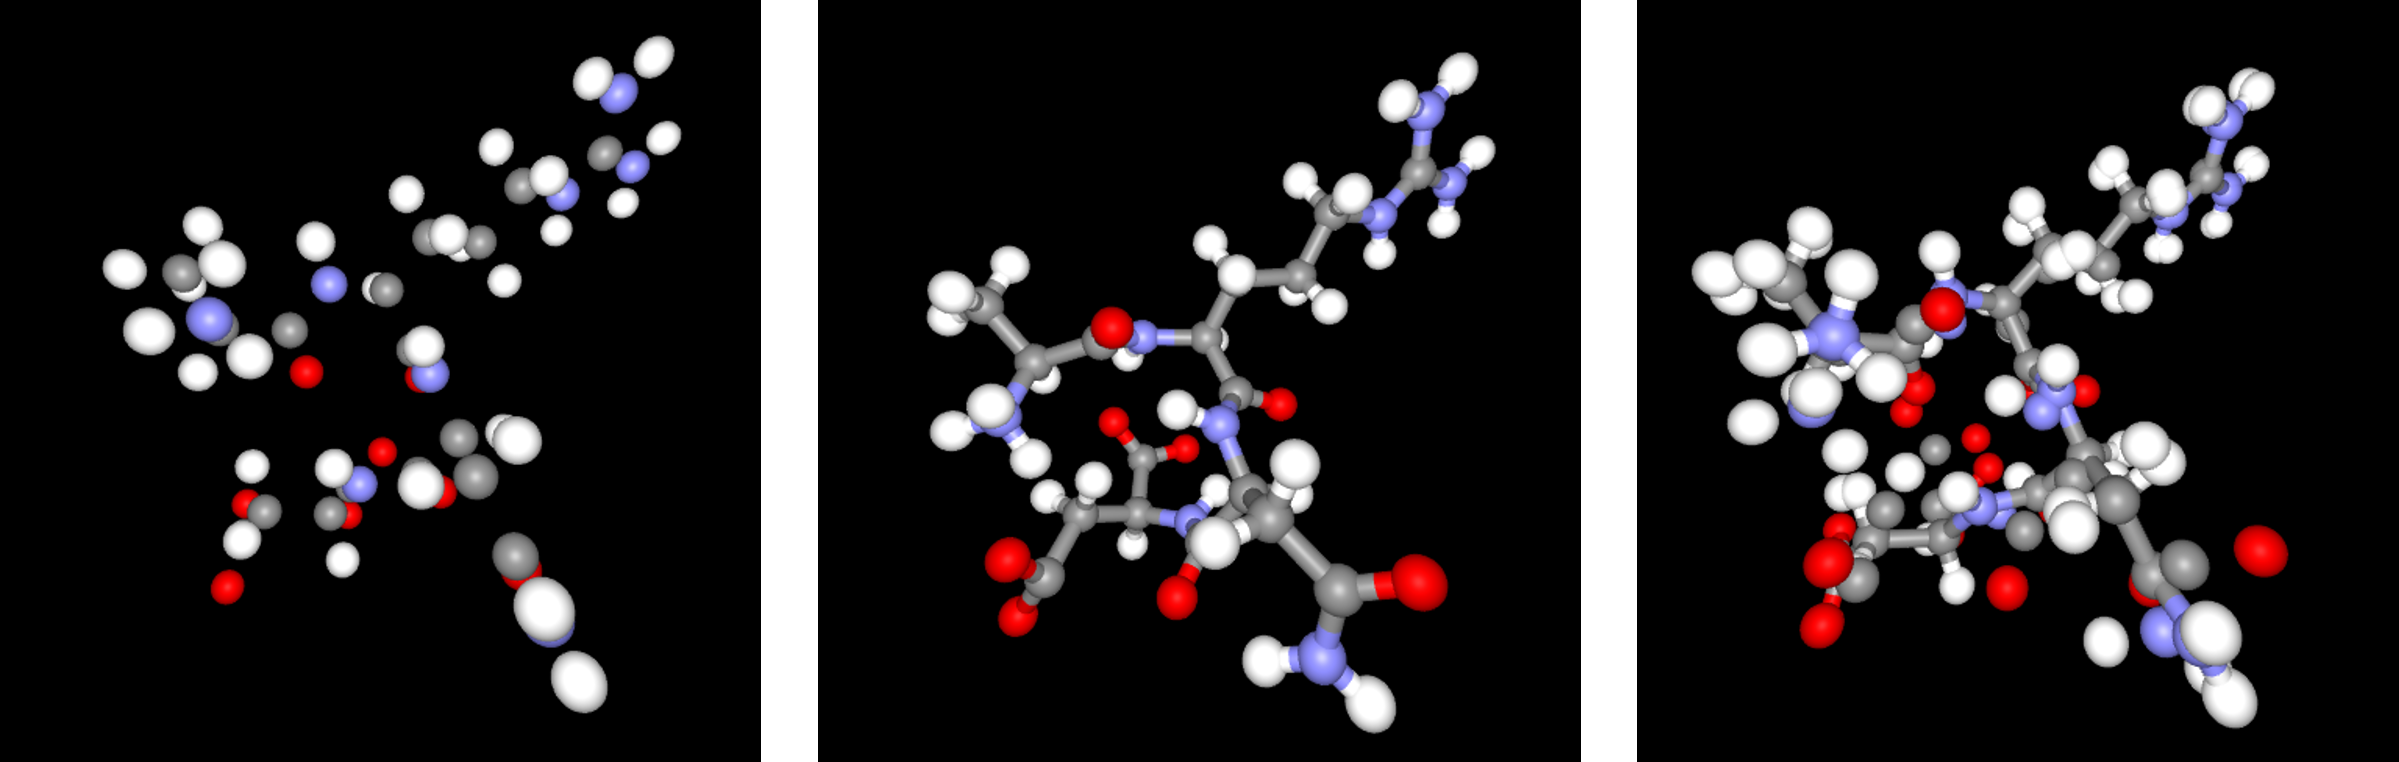
\includegraphics[width=18cm]{gfx/biovis.png}
	\caption{The \texttt{ball-and-stick}-representation of the code listing~\ref{lst:rmsd-and-amber}. The first molecule without preprocessing (\textit{left}) and after preprocessing (\textit{center}). Finally, the two structures are superposed (\textit{right}).}
	\label{fig:biochem_visualization}
\end{figure*}